\definecolor{links}{HTML}{2A1B81}
\hypersetup{colorlinks,linkcolor=,urlcolor=links}

\usetheme{Boadilla}
\usecolortheme{seahorse}
%\usefonttheme{serif}
\beamertemplatenavigationsymbolsempty

\setbeamertemplate{bibliography item}{\insertbiblabel}
\setbeamersize{description width=1cm}

\usepackage{pgfpages}
\usepackage{epigraph}
\usepackage{etoolbox}
\usepackage{tikz}
\usepackage{framed}
\usepackage[ss]{libertine}
\usepackage{amsmath}
\usepackage{mathtools}
\usepackage{listings}

%\setbeameroption{show notes on second screen=right}

\setmonofont[Ligatures=TeX]{CMU Typewriter Text}

\input{vc.tex}

\title{The Fairest Ransomware}
\author[Hikaru YOSHIMURA]{%
  Hikaru \textsc{Yoshimura}
}
\date[July 31, 2017]{%
  July 31, 2017 \\%
  {\footnotesize (Commit ID: \GITAbrHash)}
}
\institute[DWANGO Co., LTD.]{%
  DWANGO Co., Ltd.\\
  \href{mailto:yyu@mental.poker}{yyu@mental.poker}
}

\newfontfamily\quotefont[Ligatures=TeX]{Linux Libertine O} % selects Libertine as the quote font

\newcommand*\quotesize{60} % if quote size changes, need a way to make shifts relative
% Make commands for the quotes
\newcommand*{\openquote}
   {\tikz[remember picture,overlay,xshift=-4ex,yshift=-0.5ex]
   \node (OQ) {\quotefont\fontsize{\quotesize}{\quotesize}\selectfont``};\kern0pt\normalfont}

\newcommand*{\closequote}[1]
  {\tikz[remember picture,overlay,xshift=1.5ex,yshift={#1}]
   \node (CQ) {\quotefont\fontsize{\quotesize}{\quotesize}\selectfont''};}

\newcommand*\shadedauthorformat{\emph} % define format for the author argument

% Now a command to allow left, right and centre alignment of the author
\newcommand*\authoralign[1]{%
  \if#1l
    \def\authorfill{}\def\quotefill{\hfill}
  \else
    \if#1r
      \def\authorfill{\hfill}\def\quotefill{}
    \else
      \if#1c
        \gdef\authorfill{\hfill}\def\quotefill{\hfill}
      \else\typeout{Invalid option}
      \fi
    \fi
  \fi}
% wrap everything in its own environment which takes one argument (author) and one optional argument
% specifying the alignment [l, r or c]
%
\newenvironment{shadequote}[2][l]%
{\authoralign{#1}
\ifblank{#2}
   {\def\shadequoteauthor{}\def\yshift{-2ex}\def\quotefill{\hfill}}
   {\def\shadequoteauthor{\par\authorfill\shadedauthorformat{#2}}\def\yshift{2ex}}
\begin{quote}\openquote}
{\shadequoteauthor\quotefill\closequote{\yshift}\end{quote}}

\makeatletter
\def\@fnsymbol#1{\ensuremath{\ifcase#1\or *\or \dagger\or \ddagger\or
   \mathsection\or \mathparagraph\or \|\or **\or \dagger\dagger
   \or \ddagger\ddagger \else\@ctrerr\fi}}
\makeatother

\renewcommand{\thefootnote}{\fnsymbol{footnote}}

\usetikzlibrary{shapes.callouts} 

\pgfkeys{%
    /calloutquote/.cd,
    width/.code                   =  {\def\calloutquotewidth{#1}},
    position/.code                =  {\def\calloutquotepos{#1}}, 
    author/.code                  =  {\def\calloutquoteauthor{#1}},
    /calloutquote/.unknown/.code   =  {\let\searchname=\pgfkeyscurrentname
                                 \pgfkeysalso{\searchname/.try=#1,                                
    /tikz/\searchname/.retry=#1},\pgfkeysalso{\searchname/.try=#1,
                                  /pgf/\searchname/.retry=#1}}
                            }  


\newcommand\calloutquote[2][]{%
       \pgfkeys{/calloutquote/.cd,
         width               = 5cm,
         position            = {(0,-1)},
         author              = {}}
  \pgfqkeys{/calloutquote}{#1}                   
  \node [rectangle callout,callout relative pointer={\calloutquotepos},text width=\calloutquotewidth,/calloutquote/.cd,
     #1] (tmpcall) at (0,0) {\hfil#2\hfil};
  \node at (tmpcall.pointer){\calloutquoteauthor};    
}

\newfontfamily\listingfont{Menlo}
\definecolor{dkgreen}{rgb}{0,0.6,0}
\definecolor{gray}{rgb}{0.5,0.5,0.5}
\definecolor{mauve}{rgb}{0.58,0,0.82}

\makeatletter
\lst@CCPutMacro\lst@ProcessOther {"2D}{\lst@ttfamily{-{}}{-{}}}
\@empty\z@\@empty
\makeatother

\lstset{
  basicstyle=\listingfont,
  frame=single,
  xleftmargin=2em,
  xrightmargin=1em,
  breaklines=true
}

\lstdefinestyle{scala}{
  basicstyle=\listingfont\scriptsize,
  breakatwhitespace=false,
  language=scala,
  captionpos=b,
  commentstyle=\listingfont\scriptsize\color{dkgreen},
  extendedchars=true,
  xleftmargin=2em,
  xrightmargin=1em,
  keepspaces=true,
  keywordstyle=\listingfont\scriptsize\color{blue},
  emphstyle=\listingfont\scriptsize\color{cyan},
  rulecolor=\listingfont\scriptsize\color{black},
  showspaces=false,
  showstringspaces=false,
  showtabs=false,
  stringstyle=\listingfont\scriptsize\color{mauve},
  tabsize=2
}

\lstdefinelanguage{scala}{
  morekeywords={abstract,case,catch,class,def,%
    do,else,extends,false,final,finally,%
    for,if,implicit,import,match,mixin,%
    new,null,object,override,package,%
    private,protected,requires,return,sealed,%
    super,this,throw,trait,true,try,%
    type,val,var,while,with,yield},
  moreemph={Byte,Short,Int,Long,Float,Double,Char,
    String,Boolean,Unit,Null,Nothing,Any,AnyRef,
    Left,Right,Either},
  otherkeywords={=>,<-,<\%,<:,>:,\#,@},
  sensitive=true,
  morecomment=[l]{//},
  morecomment=[n]{/*}{*/},
  morestring=[b]",
  morestring=[b]',
  morestring=[b]"""
}


\newcommand\ballref[1]{%
\tikz \node[circle, shade,ball color=structure.fg,inner sep=0pt,%
  text width=8pt,font=\tiny,align=center] {\color{white}\ref{#1}};
}

\begin{document}

\frame{\maketitle}

\begin{frame}
  \frametitle{Table of Contents}

  \tableofcontents
\end{frame}

\section{Who am I?}
\begin{frame}
  \frametitle{Who am I?}
  
  \begin{columns}
    \begin{column}{0.3\textwidth}
      \centering
      \begin{figure}
        
\includegraphics[width=0.95\textwidth]{img/bird2x.png}
      \end{figure}

      \begin{description}
        \item[Twitter] \href{https://twitter.com/\_yyu\_}{@\_yyu\_}
        \item[Qiita] \href{http://qiita.com/yyu}{yyu}
        \item[GitHub] \href{https://github.com/y-yu}{y-yu}
      \end{description}
    \end{column}
    \begin{column}{0.7\textwidth}
      \begin{itemize}
        \item<2-> University of Tsukuba (Undergraduate)
        \item<3-> Authentication Platform Section, DCS Dept
        \item<4-> I'm interesting in Cryptography
      \end{itemize}
    \end{column}
  \end{columns}
\end{frame}

\section{Introduction}

\begin{frame}
  \frametitle{Introduction}

  \begin{itemize}
    \item<2-> Recentry, \emph{Ransomwares} are being famous.
  \end{itemize}

  \uncover<3->{
    \begin{block}{Ransomware}
      Ransomware is one of the malwares, which encrypts
      the data on a victim's comptuer and then make
      they pay ransom in exchange for decrypting.
    \end{block}
  }

  \uncover<4->{
    \begin{exampleblock}{Famous Ransomwares}
      \begin{itemize}
        \item WannaCry
        \item Petya
        \item GoldenEye 
      \end{itemize}
    \end{exampleblock}
  }

  \begin{center}
    \uncover<5->{
      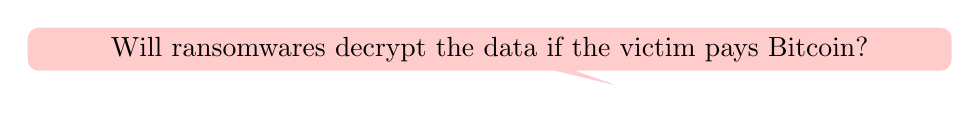
\begin{tikzpicture}
        \calloutquote[width=11.5cm,position={(0.7,-0.2)},fill=red!20,rounded corners]{Will ransomwares decrypt the data if the victim pays Bitcoin?}
      \end{tikzpicture}
    }
  \end{center} 
\end{frame}

\section{Definition and Notation}

\begin{frame}
  \frametitle{The Fairnest Ransomware}

  \uncover<2->{
    \begin{shadequote}{}
      If the victim pays some Bitcoins,
      their data will be decrypted under
      the probability on which they agreed.
    \end{shadequote}
  }

    \begin{center}
    \uncover<3->{
      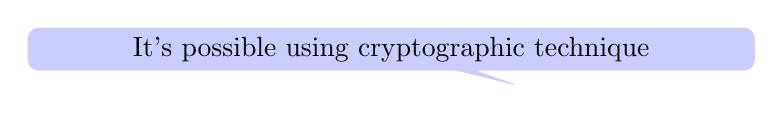
\begin{tikzpicture}
        \calloutquote[width=9cm,position={(0.7,-0.2)},fill=blue!20,rounded corners]{It's possible using cryptographic technique}
      \end{tikzpicture}
    }
  \end{center} 
\end{frame}

\newcommand{\Enc}[2]{\text{Enc}_{#1}\left(#2\right)}
\newcommand{\Dec}[2]{\text{Dec}_{#1}\left(#2\right)}

\begin{frame}
  \frametitle{Encryption}

  \begin{description}
    \item<2->[Symmetric Key Encryption (SKE)]
    is a cryptographic scheme that uses the \emph{same} key to encrypt and
    decrypt data like AES.
    An encryption function is denoted $\text{Enc}$, a decryption function
    is denoted $\text{Dec}$. The following equation holds for the symmetric key $k$.
    \[
      x = \Dec{k}{\Enc{k}{x}}
    \]
    
    \item<3->[RSA Encryption]
    is a cryptographic scheme that uses the \emph{different} keys between encrypting and
    decrypting data. The key using encryption is called \emph{public key} and
    The key using description is called \emph{secret key}.
    The following holds for a public key $(e, N)$ and the secret key $d$.
    \[
      x = (x^e)^d = (x^d)^e \pmod{N}
    \]
  \end{description}
\end{frame}

\begin{frame}
  \frametitle{Hash Function}

  \uncover<2->{
    \begin{block}{Hash Function}
      A hash function $H$ is a \emph{one way function}, which means that:
      \begin{itemize}
        \item It's easy to calculate the output $H(x)$ from input $x$
        \item But it's hard to calculate the input $x$ from output $H(x)$
      \end{itemize}
    \end{block}
  }

  \uncover<3->{
    A hash function $H$ has the following properties:
  }
  
  \begin{description}
    \item<4->[Preimage Resistance] A hash value $h$,
    it's difficult to find any message $m$ such that $h = H(m)$.

    \item<4->[Second Preimage Resistance] An input $m_1$,
    it's difficult to find different input $m_2$ such that $H(m_1) = H(m_2)$.

    \item<4->[Collision resistance] It's difficult to find
    two different messages $m_1$ and $m_2$ such that $H(m_1) = H(m_2)$.
  \end{description}
\end{frame}

\begin{frame}
  \frametitle{Zero-Knowledge Proof}

  \uncover<2->{
    There are two people, Alice and Bob.
  }

  \begin{description}
    \item<3->[Prover Alice] has the secret key $d$ for
    RSA chipher text $c$ encrypted by public key $(e, N)$.
    And she has chipher text $s := \Enc{k}{c^d \bmod N}$ and
    its symmetric key $k$.
    
    \item<4->[Verifier Bob] has the cipher text $c$,
    its public key $(e, N)$ and the cipher text $s$.
  \end{description}

  \uncover<5->{
    Bob want to verify as follows:
    
    \begin{shadequote}{}
      A preimage of the hash value $H(k)$ is a symmetric key $k$ that
      can decrypt SKE chipher text $s$.
    \end{shadequote}

    \begin{flushright}
      without knowing the secret key $d$ or symmetric key $k$.
    \end{flushright}
  }
\end{frame}

\newcommand{\ZZ}{\mathbb{Z}}

\begin{frame}[fragile]
  \frametitle{Zero-Knowledge Proof}

  We use \emph{cut-and-choose protocol} where
  RSA chipher text $c$ encrypted by public key $(e, N)$ and
  its secret key $d$.

  %\uncover<2->{
  %  \begin{center}
  %  \pseudocode{%
  %    \textbf{Alice} \< \< \textbf{Bob} \\[][\hline]
  %    \text{$F := \{\sigma_1, \dots, \sigma_n\}$}\< \< \\
  %    \text{$R := \{d_1, \dots, d_m\}$} \< \< \\
  %    \text{$\beta$ is a random permutation} \< \< \\
  %    \text{for $\{\sigma_1, \dots, \sigma_n, d_1, \dots, d_m\}$} \< \< \\
  %    \< \sendmessageright{top=$\beta$} \< \\
  %    \< \< \text{$f(\beta)$}\\
  %    \text{finalize} \< \<}
  %  \end{center}
  %}
\end{frame}
  
\begin{frame}
  \centering
  {\Huge Thank you for your attention!\\
    \vspace{1em}
    Any question?
  }
\end{frame}

\end{document}
